\subsubsection{Numerical experiments - Estimation of $\Phi$}

\textbf{Smooth case.} We consider \eqref{eq:OneDModel} with $D = \left[ -1, 1 \right]$, the final time $T = 0.5$ and we define
\begin{align}\label{eq:FunctionsOneDSmoothPhi}
\begin{split}
	f(x) &= -V'(x), \text{ where } V(x) = 8x^4 - 8x^2 + x + 2, \\
	g(x) &= \sigma = 2.
\end{split}
\end{align}
In order to approximate $\Phi$, we perform a Montecarlo simulation using both DEM and CEM, with $M = 6 \cdot 10^5$ trajectories in order to kill the statistical error. We consider the number of timesteps for the time integration to be $N = 2^i, i = 5, \dots, 12$. Numerical results (Figure \ref{fig:KillOneDPhi}) confirm that the weak error for DEM is of order 0.5, while for CEM the order of convergence is 1.

\begin{figure}[t]
    \centering
    \begin{subfigure}{0.49\linewidth}
        \centering
        \resizebox{1\linewidth}{!}{% This file was created by matlab2tikz.
%
%The latest updates can be retrieved from
%  http://www.mathworks.com/matlabcentral/fileexchange/22022-matlab2tikz-matlab2tikz
%where you can also make suggestions and rate matlab2tikz.
%
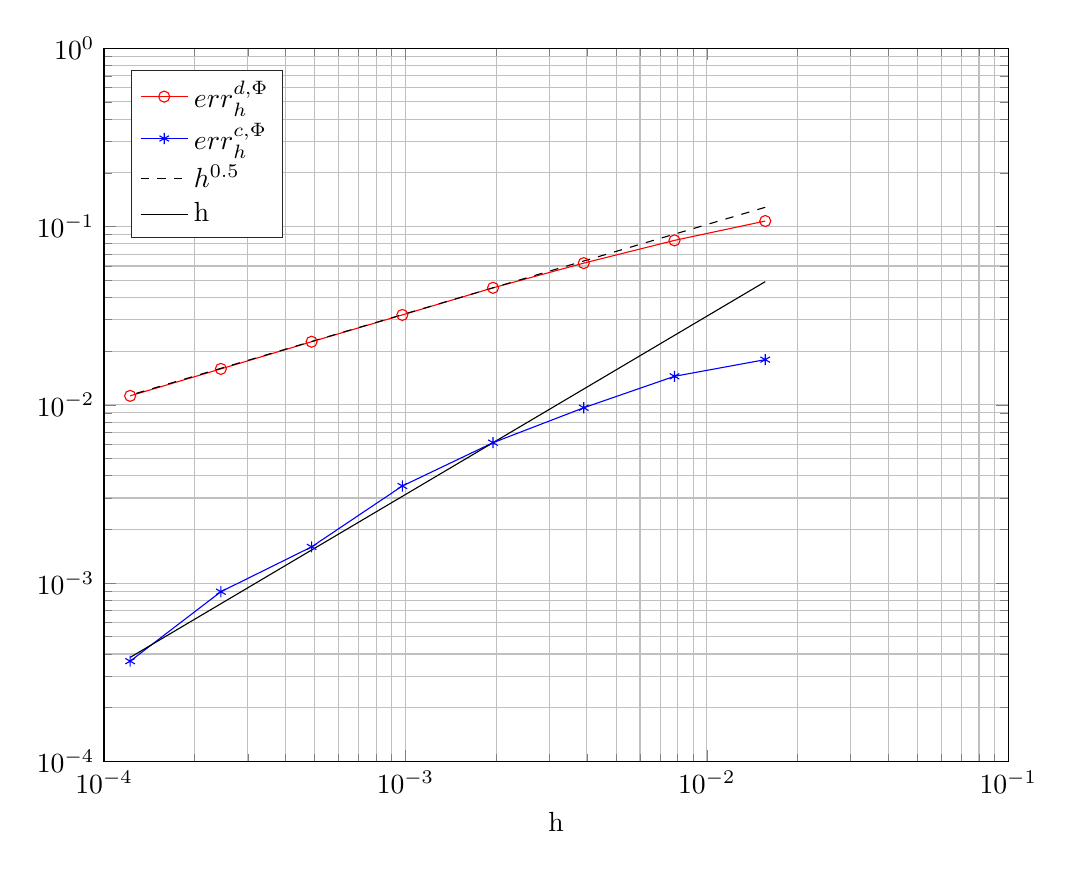
\begin{tikzpicture}

\begin{axis}[%
width=4.521in,
height=3.566in,
at={(0.758in,0.481in)},
scale only axis,
xmode=log,
xmin=0.0001,
xmax=0.1,
xminorticks=true,
xlabel={h},
xmajorgrids,
xminorgrids,
ymode=log,
ymin=0.0001,
ymax=1,
yminorticks=true,
ymajorgrids,
yminorgrids,
axis background/.style={fill=white},
legend style={at={(0.03,0.97)},anchor=north west,legend cell align=left,align=left,draw=white!15!black}
]
\addplot [color=red,solid,mark=o,mark options={solid}]
  table[row sep=crcr]{%
0.015625	0.107253818761899\\
0.0078125	0.083570485428566\\
0.00390625	0.0623038187618994\\
0.001953125	0.0452871520952327\\
0.0009765625	0.0319088187618994\\
0.00048828125	0.0225721520952327\\
0.000244140625	0.0158938187618994\\
0.0001220703125	0.011220485428566\\
};
\addlegendentry{$\text{err}_\text{h}^{\text{d,}\Phi}$};

\addplot [color=blue,solid,mark=asterisk,mark options={solid}]
  table[row sep=crcr]{%
0.015625	0.0179128479047673\\
0.0078125	0.0144461812381006\\
0.00390625	0.00962451457143397\\
0.001953125	0.00612951457143396\\
0.0009765625	0.00350451457143397\\
0.00048828125	0.00159618123810062\\
0.000244140625	0.000894514571433969\\
0.0001220703125	0.000364838190478001\\
};
\addlegendentry{$\text{err}_\text{h}^{\text{c,}\Phi}$};

\addplot [color=black,dashed]
  table[row sep=crcr]{%
0.015625	0.128091409388663\\
0.0078125	0.0905743041904655\\
0.00390625	0.0640457046943313\\
0.001953125	0.0452871520952327\\
0.0009765625	0.0320228523471656\\
0.00048828125	0.0226435760476164\\
0.000244140625	0.0160114261735828\\
0.0001220703125	0.0113217880238082\\
};
\addlegendentry{$\text{h}^{\text{0.5}}$};

\addplot [color=black,solid]
  table[row sep=crcr]{%
0.015625	0.0490361165714717\\
0.0078125	0.0245180582857358\\
0.00390625	0.0122590291428679\\
0.001953125	0.00612951457143396\\
0.0009765625	0.00306475728571698\\
0.00048828125	0.00153237864285849\\
0.000244140625	0.000766189321429245\\
0.0001220703125	0.000383094660714622\\
};
\addlegendentry{h};

\end{axis}
\end{tikzpicture}% }  
        \caption{Killing boundary in $x = 1$}
        \label{fig:KillOneDPhi}
    \end{subfigure}
    \begin{subfigure}{0.49\linewidth}
        \centering
        \resizebox{1\linewidth}{!}{% This file was created by matlab2tikz.
%
%The latest updates can be retrieved from
%  http://www.mathworks.com/matlabcentral/fileexchange/22022-matlab2tikz-matlab2tikz
%where you can also make suggestions and rate matlab2tikz.
%
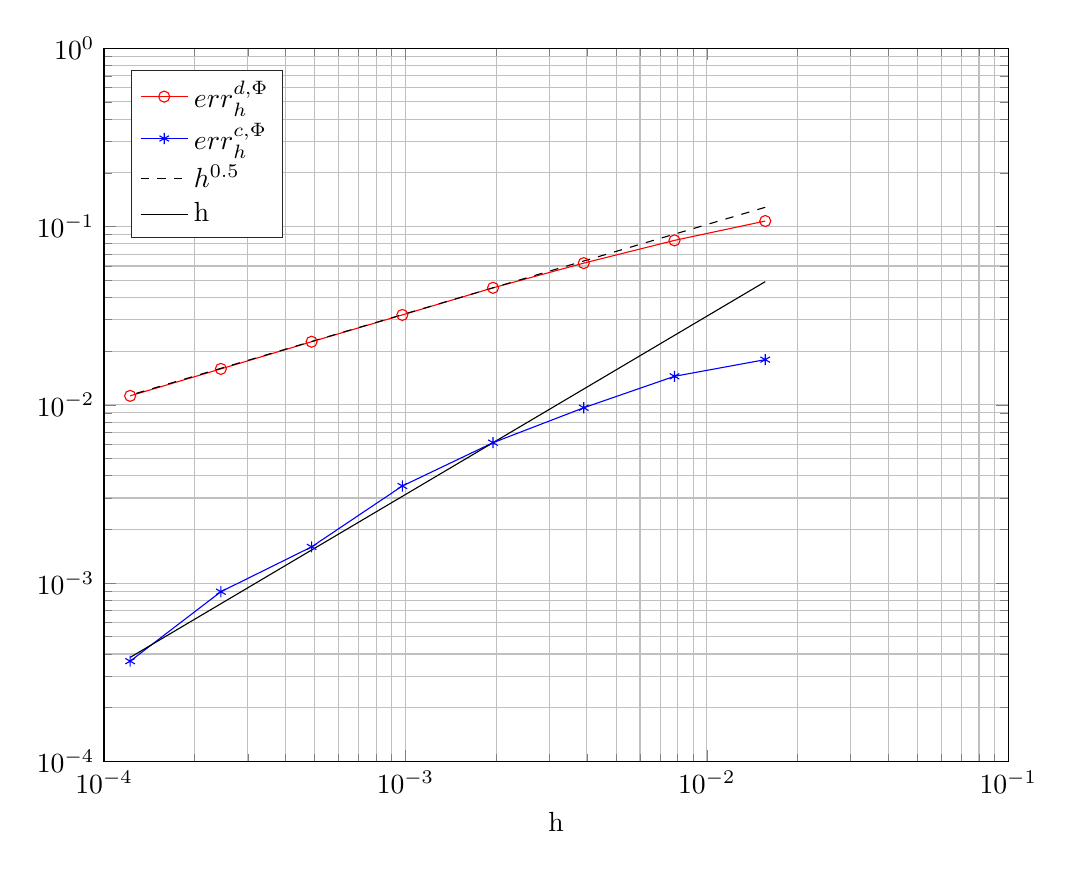
\begin{tikzpicture}

\begin{axis}[%
width=4.521in,
height=3.566in,
at={(0.758in,0.481in)},
scale only axis,
xmode=log,
xmin=0.0001,
xmax=0.1,
xminorticks=true,
xlabel={h},
xmajorgrids,
xminorgrids,
ymode=log,
ymin=0.0001,
ymax=1,
yminorticks=true,
ymajorgrids,
yminorgrids,
axis background/.style={fill=white},
legend style={at={(0.03,0.97)},anchor=north west,legend cell align=left,align=left,draw=white!15!black}
]
\addplot [color=red,solid,mark=o,mark options={solid}]
  table[row sep=crcr]{%
0.015625	0.107253818761899\\
0.0078125	0.083570485428566\\
0.00390625	0.0623038187618994\\
0.001953125	0.0452871520952327\\
0.0009765625	0.0319088187618994\\
0.00048828125	0.0225721520952327\\
0.000244140625	0.0158938187618994\\
0.0001220703125	0.011220485428566\\
};
\addlegendentry{$\text{err}_\text{h}^{\text{d,}\Phi}$};

\addplot [color=blue,solid,mark=asterisk,mark options={solid}]
  table[row sep=crcr]{%
0.015625	0.0179128479047673\\
0.0078125	0.0144461812381006\\
0.00390625	0.00962451457143397\\
0.001953125	0.00612951457143396\\
0.0009765625	0.00350451457143397\\
0.00048828125	0.00159618123810062\\
0.000244140625	0.000894514571433969\\
0.0001220703125	0.000364838190478001\\
};
\addlegendentry{$\text{err}_\text{h}^{\text{c,}\Phi}$};

\addplot [color=black,dashed]
  table[row sep=crcr]{%
0.015625	0.128091409388663\\
0.0078125	0.0905743041904655\\
0.00390625	0.0640457046943313\\
0.001953125	0.0452871520952327\\
0.0009765625	0.0320228523471656\\
0.00048828125	0.0226435760476164\\
0.000244140625	0.0160114261735828\\
0.0001220703125	0.0113217880238082\\
};
\addlegendentry{$\text{h}^{\text{0.5}}$};

\addplot [color=black,solid]
  table[row sep=crcr]{%
0.015625	0.0490361165714717\\
0.0078125	0.0245180582857358\\
0.00390625	0.0122590291428679\\
0.001953125	0.00612951457143396\\
0.0009765625	0.00306475728571698\\
0.00048828125	0.00153237864285849\\
0.000244140625	0.000766189321429245\\
0.0001220703125	0.000383094660714622\\
};
\addlegendentry{h};

\end{axis}
\end{tikzpicture}% }  
        \caption{Reflecting boundary in $x = 1$}
        \label{fig:ReflectOneDPhi}
    \end{subfigure}    
    \caption{Approximation of $\Phi$. Orders of convergence of DEM and CEM in the one-dimensional case.}
    \label{fig:OrdersOneDPhi}
\end{figure}


